\stopallthesefloats
\subsection{Cache Coloring to Curtain Interference}
\begin{figure}[hbt]
\begin{center}
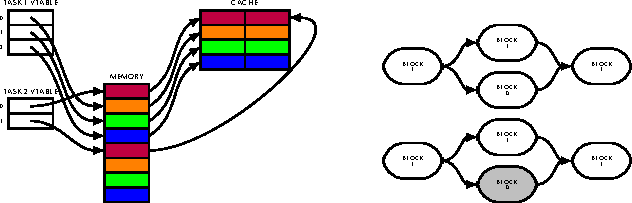
\includegraphics[width=\textwidth]{\chapterdirectory/figure/handling_it/cache_coloring_wcet.pdf}
\end{center}
\caption{Cache coloring aware scheduling, from \cite{DBLP:journals/corr/abs-1903-09310}}%
\label{fig:handling_it:cache_coloring}
\end{figure}
When using a set-associative cache, the cache is divided in equal sets of cache
lines. The memory element's physical address determines which of these sets of
cache lines it will go to. The cache eviction policy then applies solely inside
that set. The idea behind cache coloring is to exploit this, by determining
which memory element will find itself in which set of lines, and assigning
virtual addresses to physical addresses in a manner that will ensure a maximum
of virtual addresses will find themselves in the cache.

\cite{DBLP:journals/corr/abs-1903-09310} uses cache coloring in the opposite
manner. It instead assigns a single color (thus, set of cache lines) per
program. While this is not an efficient use of the cache for any one program,
it means that each program is effectively curtained into the set of caches of
its color. Using careful scheduling, the number of programs running in parallel
that share the same colors can be reduced (see
Figure~\ref{fig:handling_it:cache_coloring}), thus removing the interference
they can inflict on one another.
\stopallthesefloats
